\chapter{Конструкторский раздел}
В этом разделе будут приведены схемы реализации алгоритмов,
а также выбранные классы эквивалентности для тестирования ПО.

\section{Схемы алгоритмов}
На рисунке 2.1 будет приведена схема реализации алгоритма полного перебора.

На рисунке 2.2 будет приведена схема реализации алгоритма бинарного поиска.

На рисунке 2.3 будет приведена схема реализации алгоритма поиска с использованием сегментов.

\FloatBarrier
\begin{figure}[hp]
	\begin{center}
		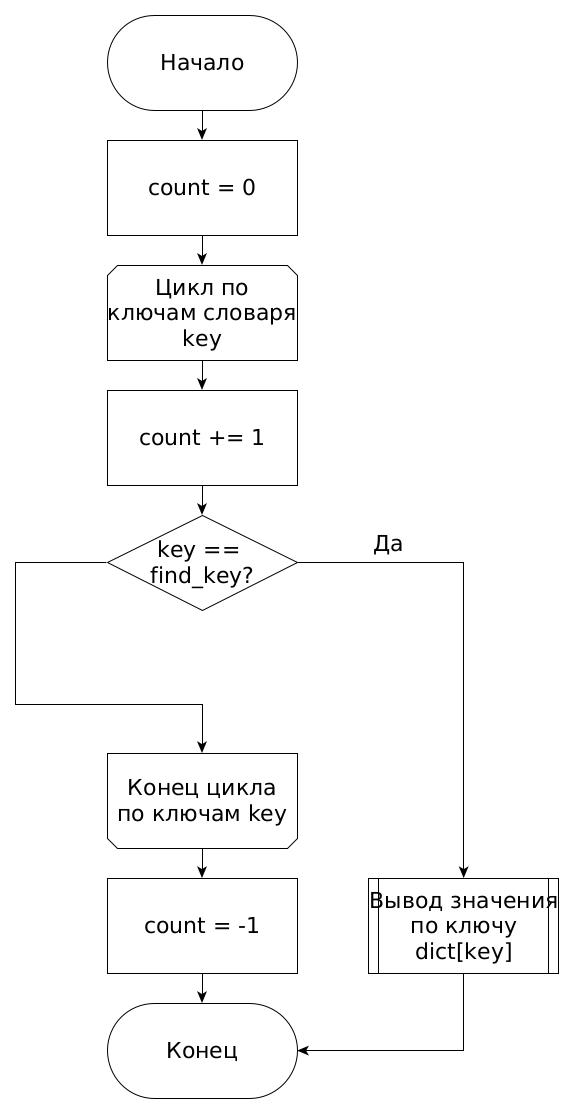
\includegraphics[width=11cm, height=23cm]{graph/full.jpg}
	\end{center}
	\caption{Схема реализации алгоритма полного перебора}
\end{figure}
\FloatBarrier

\FloatBarrier
\begin{figure}[hp]
	\begin{center}
		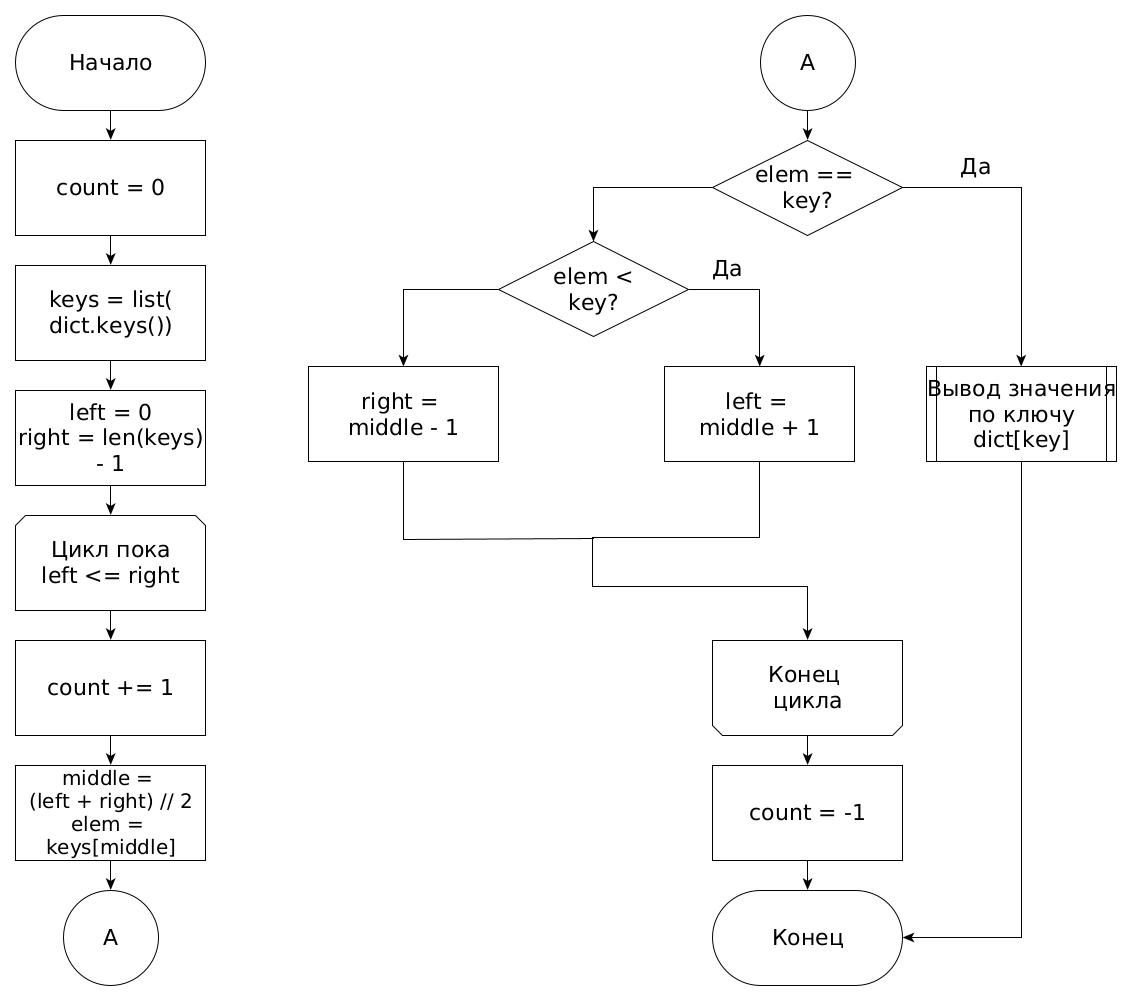
\includegraphics[width=\linewidth]{graph/binary.jpg}
	\end{center}
	\caption{Схема реализации алгоритма бинарного поиска}
\end{figure}
\FloatBarrier

\FloatBarrier
\begin{figure}[hp]
	\begin{center}
		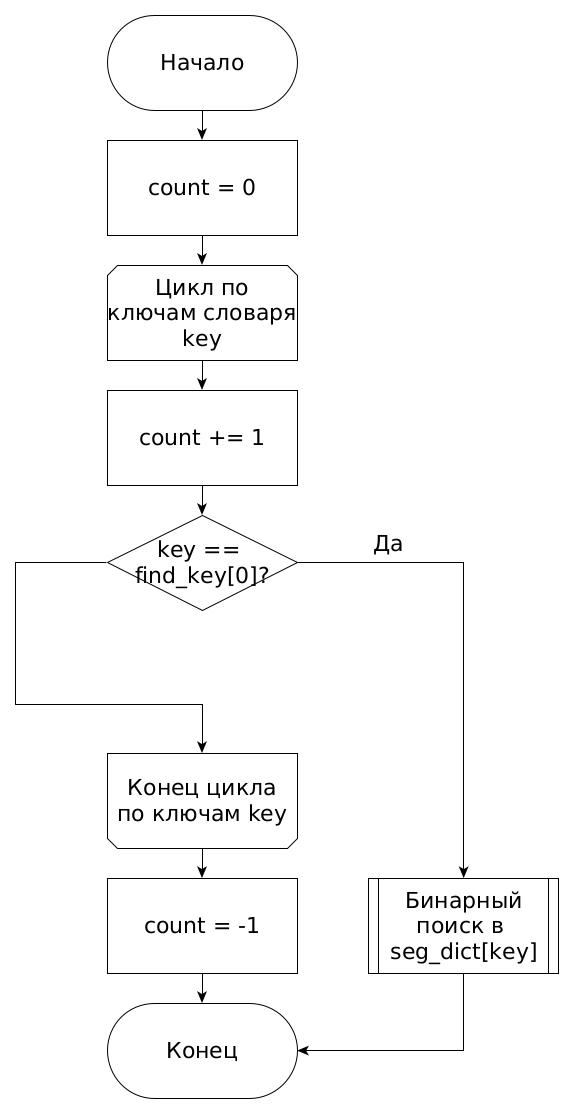
\includegraphics[width=11cm, height=23cm]{graph/segment.jpg}
	\end{center}
	\caption{Схема реализации поиска с использованием сегмента}
\end{figure}
\FloatBarrier

\section{Типы данных для алгоритмов}
Для реализации алгоритма будет использоваться тип данных dict из python.
Ключ -- номер паспорта, является строковой переменной.
Значение ключа -- список, состоящий из трёх строковых переменных, соответствующих ФИО.

\section{Способ тестирования}
Тестирование программы будет произодиться методом чёрного ящика.
Такой подход выбран, так как от реализаций алгоритмов требуется в первую
очередь правильность работы.
Сама по себе реализация не требует тестировки, так как в точности
повторяет теоретические принципы, сформированные в аналитическом
разделе.

В качестве классов эквивалентности были выбраны следующие сущности:
\begin{itemize}
	\item ключ, которого нет в словаре;
	\item ключ, который есть в словаре;
	\item ключ, который является первым в словаре;
	\item ключ, который является последним в словаре.
\end{itemize}

\section{Вывод}
Были приведены схемы реализации алгоритмов и типы данных для алгоритмов.
Был определен способ тестирования алгоритмов.